\chapter{\texttt{NP} completezza e \texttt{co-NP}}
\section{Classi di complessità}
L'idea fondamentale per dimostrare che determinati problemi sono più difficili dei problemi 
risolvibili in tempo polinomiale è quella di ``ritagliare'' una classe di problemi
che abbiano una determinata caratteristica, e dimostrare che un problema specifico
è almeno tanto difficile quanto i problemi di quella classe, \textbf{riducendo} il problema
specifico ad un problema della classe.
\subsection{Tipologie di problemi}
\begin{itemize}
    \item \textbf{Problemi decisionali}: problemi che ammettono risposta
    sì/no. Un problema di decisione è quindi un insieme di istanze, e la risposta
    è sì se l'istanza appartiene all'insieme, no altrimenti.

    \textit{Un problema di decisione è il seguente: dato un grafo $\mathcal{G}$ dire se 
    esiste un cammino euleriano in $\mathcal{G}$.}

    \item \textbf{Problemi di ricerca}: problemi di ricerca ammettono una soluzione
    che può essere trovata in tempo polinomiale.

    \textit{Un problema di ricerca è il seguente: dato un grafo $\mathcal{G}$
    trovare un cammino euleriano in $\mathcal{G}$.}
            
    \item \textbf{Problemi di ottimizzazione}: problemi di ottimizzazione
    ammettono una soluzione che può essere trovata in tempo polinomiale.

    \textit{Un problema di ottimizzazione è il seguente: dato un grafo $\mathcal{G}$
    trovare il cammino euleriano più lungo in $\mathcal{G}$.}
\end{itemize}
Nello studio della complessità considereremo solo problemi decisionali, in quanto
tutti i problemi di ricerca e di ottimizzazione possono essere ricondotti a problemi
di decisione. Ciò significa che se siamo in grado di dire che un determinato problema
di decisione è difficile, allora possiamo dire che anche il problema di ricerca e
quello di ottimizzazione sono difficili, perché se fossimo in grado di risolvere un 
problema di ricerca o di ottimizzazione, potremmo risolvere anche il problema di decisione
in tempo polinomiale.
\subsection{Formalizzazione di un problema computazionale}
In relazione a ciò che è stato detto nella sezione \ref{sec:problema_computazionale}, 
un problema computazionale è un insieme infinito di istanze e la loro relazione con
la soluzione associata. Matematicamente, possiamo definire un problema computazionale
attraverso:
\begin{itemize}
    \item $\mathbb{A}$ denota il problema computazionale sotto esame.
    \item $\mathscr{I}(\mathbb{A})$ rappresenta lo spazio delle istanze,
    ovvero il dominio dei possibili quesiti.
    \item $\texttt{sol}(\mathbb{A})$ esprime la relazione che associa a
    ciascuna istanza la sua soluzione o insieme di soluzioni.
\end{itemize}

\begin{exmp}
Consideriamo, ad esempio, il problema del ciclo hamiltoniano. In questo contesto:
    \begin{itemize}
        \item $\mathbb{A}$ corrisponde alla questione di determinare l'esistenza
        di un ciclo hamiltoniano.
        \item $\mathscr{I}(\mathbb{A})$ comprende tutti i possibili grafi $\mathcal{G}$
        sui quali indaghiamo.
        \item $\texttt{sol}(\mathbb{A})$ identifica i percorsi che visitano ogni nodo del
        grafo esattamente una volta, se esistenti.
    \end{itemize}
\end{exmp}

Pertanto, la relazione $\mathbb{A}$ si configura come una \textbf{connessione} fra lo
spazio delle istanze e le corrispondenti soluzioni. Matematicamente, ciò si traduce
nella seguente inclusione:
\[ \mathbb{A} \subseteq \mathscr{I}(\mathbb{A}) \times \texttt{sol}(\mathbb{A}) \]
indicando con $(\mathcal{G}, \mathcal{P})$ l'insieme delle coppie dove $\mathcal{P}$
rappresenta un valido ciclo hamiltoniano nel grafo $\mathcal{G}$.

Per ciascuna istanza $x$ appartenente allo spazio dei problemi computazionali,
$\texttt{sol}(x)$ denota l'insieme delle soluzioni $y$ tali che $(x, y) \in \mathbb{A}$,
ovvero:
\[
    \texttt{sol}(x) = \{ y \mid (x, y) \in \mathbb{A} \}
\]

\subsubsection{Problemi di Decisione}
Nei problemi di decisione, lo spazio delle soluzioni è binario, $\texttt{sol}(\mathbb{A})
= \{ \texttt{yes}, \texttt{no} \}$. Pertanto, $A$ associa a ciascuna istanza $x$ una delle
due possibili risposte, determinando se l'istanza soddisfa la proprietà esaminata:
\[
    A : \mathscr{I}(\mathbb{A}) \rightarrow \{ \texttt{yes}, \texttt{no} \}
\]

\subsubsection{Problemi di Ricerca}
Per i problemi di ricerca $\mathbb{A}^S$, il problema di decisione associato $\mathbb{A}^D$
verifica l'esistenza di almeno una soluzione per l'istanza $x$:
\[
    \mathbb{A}^D(x) = 
    \begin{cases}
        \texttt{yes} & \text{se esiste almeno una soluzione}, \\
        \texttt{no} & \text{altrimenti}
    \end{cases}
\]

\subsection{La Classe \texttt{P}}

Nella teoria della complessità computazionale, la capacità di risolvere un problema
computazionale va oltre la semplice identificazione di una soluzione per un'istanza
specifica. Ciò richiede l'impiego di un algoritmo deterministico $A$ che, per ogni istanza
$x$ nell'insieme $\mathscr{I}(\mathbb{A})$, produce una soluzione $y$ valida, ovvero $y
\in \texttt{sol}(x)$:
\[
  A(x) = y \quad \text{con} \quad y \in \texttt{sol}(x)
\]

Il \textit{tempo di esecuzione} $T_A(x)$ dell'algoritmo $A$ su un'istanza $x$ è fondamentale,
poiché riflette l'efficienza con cui l'algoritmo raggiunge la soluzione.

\begin{tcolorbox}[title={Classe \texttt{P}}]
Un algoritmo $A$ è definito \textit{polinomiale} (\texttt{poly-time}) quando il suo tempo di
esecuzione, per ogni istanza $x \in \mathscr{I}(\mathbb{A})$, è limitato superiormente da
un polinomio nella dimensione di $x$:
\[
    T_A(x) = O(|x|^c) \quad \text{per una certa costante } c \in \mathbb{N}.
\]
\end{tcolorbox}

Un problema computazionale viene considerato \textit{fuori dalla classe \texttt{P}} qualora
non esista, per nessuna costante $c$, un algoritmo capace di risolvere tutte le sue istanze
in tempo polinomiale $O(n^c)$.

\subsection{La Classe \texttt{EXP}}
\begin{tcolorbox}[title={Classe \texttt{EXP}}]
    La classe \texttt{EXP} raggruppa i problemi di decisione risolvibili da un algoritmo
    deterministico in tempo esponenziale rispetto
    alla dimensione dell'input. Un problema $\mathbb{A}$ appartiene a \texttt{EXP} se
    esiste un algoritmo $A$ per cui, data una costante $c_A$, per ogni istanza $x \in
    \mathscr{I}(\mathbb{A})$ si ha che:
    \[
        T_A(x) = O(2^{|x|^{c_A}})
    \]
    In altre parole, il tempo di esecuzione di $A$ è limitato superiormente da una
    funzione esponenziale della dimensione dell'input elevata a una costante. Questa
    classe include quindi problemi per i quali la risoluzione richiede una quantità di
    tempo che cresce esponenzialmente con l'aumentare della dimensione dell'input.
\end{tcolorbox}
Da qui segue che la classe \texttt{EXP} è una generalizzazione della classe \texttt{P},
poiché ogni problema risolvibile in tempo polinomiale è anche risolvibile in tempo
esponenziale. In altre parole, \texttt{P} è un sottoinsieme di \texttt{EXP}.
\[ \texttt{P} \subseteq \texttt{EXP} \]
Perché se un problema $\mathcal{A} \in \texttt{P}$, allora esiste un algoritmo $A$, 
per cui, data una costante $c_A$, per ogni istanza $x \in \mathscr{I}(\mathbb{A})$ si ha che:
\[ T_A(x) = O(|x|^{c_A}) \]
Poiché, ogni polinomio è anche una funzione esponenziale, si ha che:
\[ T_A(x) = O(2^{|x|^{c_A}}) \]
Quindi $\mathbb{A} \in \texttt{EXP}$.

È importante notare che un problema è nella classe \texttt{EXP}, non se gli unici 
algoritmi conosciuti per risolverlo sono esponenziali, ma se esiste almeno un algoritmo
deterministico che lo risolve in tempo esponenziale.
\begin{exmp}
    Consideriamo il problema del cammino euleriano. Un cammino euleriano è un cammino che
    attraversa ogni arco del grafo esattamente una volta. 
    In input si ha un grafo $\mathcal{G}$ e si vuole sapere se esiste un cammino euleriano
    in $\mathcal{G}$, quindi l'output è \texttt{yes} se esiste un cammino euleriano e
    \texttt{no} altrimenti. 
    Questo problema è nella classe \texttt{P}, infatti esiste un algoritmo polinomiale
    per risolverlo, controllando se il grafo è connesso e se ogni nodo ha grado pari.
\end{exmp}
\begin{exmp}
    Consideriamo il problema del commesso viaggiatore. In input si ha un grafo completo
    pesato $\mathcal{G}$ e si vuole sapere se esiste un ciclo hamiltoniano di peso minimo
    in $\mathcal{G}$, quindi l'output è \texttt{yes} se esiste un ciclo hamiltoniano e
    \texttt{no} altrimenti. 
    Non sappiamo se esiste un algoritmo polinomiale per risolvere questo problema, quindi
    non sappiamo se è nella classe \texttt{P}. Sappiamo che per ogni istanza, se la soluzione 
    è \texttt{yes} possiamo certificarla in tempo polinomiale. 
\end{exmp}

\begin{tcolorbox}[title={Prova Semplice}]
    Una \textbf{prova semplice} è un certificato di lunghezza polinomiale che può essere
    verificato in tempo polinomiale. 
\end{tcolorbox}
Cerchiamo di caratterizzare i problemi che hanno una prova semplice.
\subsection{La Classe \texttt{NP}}

\begin{tcolorbox}[title = {Classe \texttt{NP}}]
    Un problema $\mathbb{A}$ appartiene alla classe \texttt{NP} se esiste un algoritmo
    deterministico $A$ (\textit{verificatore}) e una funzione polinomiale $p$ tale che, per ogni istanza $x \in
    \mathscr{I}(\mathbb{A})$, esiste un certificato $y$ di lunghezza polinomiale rispetto
    alla dimensione di $x$ tale che:
    \[
        B(x, y) = \begin{cases}
            \texttt{yes} & \text{se } x \in \texttt{sol}(\mathbb{A}), \\
            \texttt{no} & \text{altrimenti}
        \end{cases}
    \]

    Inoltre, esiste una costante $c_A$ tale che il tempo di esecuzione di $A$ è limitato
    superiormente da una funzione polinomiale della dimensione di $x$:
    \[
        T_A(x, y) = O(p(|x|^{c_A}))
    \]

    In notazione formale, si ha che:
    \begin{align*}
        \texttt{NP} = \{ &\mathbb{A} \mid \exists A, c_A,
        \forall x \in \mathscr{I}(\mathbb{A}): \mathbb{A}(x) = \texttt{yes} \Rightarrow \\
        &\exists y, |y| = O((|x|^{c_A})), \text{ t.c. } A(x, y) = \texttt{yes} \land T_A(x, y) 
        = O((|x|^{c_A})) \}
    \end{align*}
\end{tcolorbox}
È importante notare che il tempo di esecuzione del verificatore $A$ è polinomiale rispetto 
alla dimensione dell'input $x$ e del certificato $y$. Ciò significa che, se esiste un
certificato $y$ tale che $A(x, y) = \texttt{yes}$, allora esiste un algoritmo che può
verificare la soluzione in tempo polinomiale. Da questo segue che il certificato deve 
essere di lunghezza polinomiale rispetto alla dimensione dell'input $x$.
\[
    |y| = O((|x|^{c_A}))  
\]

\begin{theorem}
    La classe \texttt{P} è un sottoinsieme della classe \texttt{NP}.
    \[
        \texttt{P} \subseteq \texttt{NP}.
    \]
\end{theorem}
\begin{proof}
    Consideriamo il problema $\mathbb{A} \in \texttt{P}$. Allora esiste un algoritmo 
    deterministico $A$ che risolve per ogni istanza $x \in \mathscr{I}(\mathbb{A})$ in
    tempo polinomiale:
    \[
        T_A(x) = O(|x|^{c_A}).
    \]
    Definiamo un verificatore $B$ per $\mathbb{A}$. Per ogni istanza
    $x \in \mathscr{I}(\mathbb{A})$ e $y$, $B(x, y) = A(x)$. 
    Quindi se $\mathbb{A}(x) = \texttt{yes}$, allora per ogni $y \in \{0,1\}^*$,
    $B(x, y) = \texttt{yes}$ e se $\mathbb{A}(x) = \texttt{no}$, allora per ogni
    $y \in \{0,1\}^*$, $B(x, y) = \texttt{no}$.
\end{proof}

\begin{theorem}
    La classe \texttt{NP} è sottoinsieme della classe \texttt{EXP}.
    \[
        \texttt{NP} \subseteq \texttt{EXP}.
    \]
\end{theorem}
\begin{proof}
    Consideriamo un problema $\mathbb{A} \in \texttt{NP}$. Allora esiste un algoritmo
    deterministico $B$ e una costante $c_B$ tale che per ogni istanza $x \in
    \mathscr{I}(\mathbb{A})$, esiste un certificato $y$ di lunghezza polinomiale rispetto
    alla dimensione di $x$ tale che:
    \[
        B(x, y) = \begin{cases}
            \texttt{yes} & \text{se } x \in \texttt{sol}(\mathbb{A}), \\
            \texttt{no} & \text{altrimenti}.
        \end{cases}
    \]
    Quindi il tempo di esecuzione di $B$ è limitato superiormente da una funzione polinomiale
    della dimensione di $x$:
    \[
        T_B(x, y) = O((|x|^{c_B}))
    \]
    Definiamo un algoritmo deterministico $A^{\texttt{EXP}}$ che per ogni 
    $x \in \mathscr{I}(\mathbb{A})$ cicla su tutti i possibili certificati $y$ della 
    taglia ammissibile per i certificati e usa $B(x, y)$ per verificare se $x$ è 
    una soluzione di $\mathbb{A}$:

    \begin{algorithm}[H]
        \DontPrintSemicolon
        \caption{Algoritmo $A^{\texttt{EXP}}$}
        \KwIn{Un'istanza $x \in \mathscr{I}(\mathbb{A})$}
        \KwOut{\texttt{yes} se $x \in \texttt{sol}(\mathbb{A})$, \texttt{no} altrimenti}
        \ForEach{$y \in \{0,1\}^{|x|^{c_B}}$}{
            \If{$B(x, y) = \texttt{yes}$}{
                \Return{\texttt{yes}}
            }
            \Return{\texttt{no}}
        }
    \end{algorithm}
    Sappiamo che $A^{\texttt{EXP}}(x) = \texttt{yes}$ se e solo se esiste un certificato
    $y \in \{0,1\}^{|x|^{c_B}}$ tale che $B(x, y) = \texttt{yes}$, ovvero se 
    $\mathbb{A} = \texttt{yes}$. Il tempo di esecuzione di $A^{\texttt{EXP}}$ è limitato
    superiormente da una funzione esponenziale della dimensione di $x$:
    \[
        T_{A^{\texttt{EXP}}}(x) = O(2^{|x|^{c_B}})
    \]
    Quindi $\mathbb{A} \in \texttt{EXP}$, ovvero $\texttt{NP} \subseteq \texttt{EXP}$.
\end{proof}

\begin{figure}[H]
    \centering
    \cclasses{\texttt{EXP}, \texttt{NP}, \texttt{P}}
\end{figure}
Non sappiamo se le inclusioni sono strette, ma sappiamo che \texttt{P} è incluso
strettamente in \texttt{EXP}.

\begin{tcolorbox}[title = {Congettura $\texttt{P} \neq \texttt{NP}$}]
    Se $\texttt{P} \neq \texttt{NP}$, quindi $\texttt{P} \subset \texttt{NP}$, allora
    esistono problemi che possono essere verificati in tempo polinomiale, ma non possono
    essere risolti in tempo polinomiale.
    \begin{align*}
        \texttt{P} &\subset \texttt{NP} \\
        \texttt{P} &\neq \texttt{NP}
    \end{align*}
    Il problema è che non esiste una dimostrazione formale che 
    $\texttt{P} \neq \texttt{NP}$. Siamo convinti di ciò perché crediamo che alcuni
    problemi \texttt{NP} siano
    più difficili di altri e se siamo in grado di risolvere tali problemi allora 
    siamo in grado di risolvere tutti i problemi \texttt{NP}. Questa situazione
    porta alla distinzione tra i problemi \texttt{NP} cosiddetti ``difficili" o
    \texttt{NP-hard} e i problemi \texttt{NP-completi}, per i quali una soluzione
    efficiente implicherebbe la possibilità di risolvere efficientemente ogni problema
    nell'insieme \texttt{NP}.

\end{tcolorbox}
\begin{figure}[H]
    \centering
    \begin{tikzpicture}[set/.style={draw, circle, inner sep=0pt, align=center}]
        \node[set, fill=gray!40, text width=2.5cm] (P) at (0,0) {Problemi \texttt{P}};
        \node[set, fill=gray!40, text width=2.5cm] (NP) at (3,0) {\texttt{NP}-Completi};
        \begin{pgfonlayer}{background}
            \node[fill=gray!20, fit=(P) (NP), draw, rounded corners=0.5cm, inner
            sep=0.5cm, label={above: Problemi \texttt{NP}}] {};
        \end{pgfonlayer}
    \end{tikzpicture}
\end{figure}
\section{Riduzione polinomiale tra problemi}
La riduzione polinomiale ci permette di mettere in relazione i problemi tra loro, 
permettendoci di dimostrare che un problema è almeno tanto difficile quanto un altro
problema.
\begin{tcolorbox}[title = {Riduzione polinomiale (Karp)}]
    Siano $\mathbb{A}$ e $\mathbb{B}$ due problemi decisionali. Diciamo che $\mathbb{A}$
    si riduce polinomialmente a $\mathbb{B}$, e scriviamo $\mathbb{A} \leq_p \mathbb{B}$,
    se esiste una funzione calcolabile in tempo polinomiale $f: \{0,1\}^* \rightarrow
    \{0,1\}^*$ tale che per ogni $x \in \{0,1\}^*$:
    \[
        \forall x \in \mathbb{A} \qquad \mathbb{A}(x) = \texttt{yes} \iff \mathbb{B}(f(x)) = \texttt{yes}
    \]
\end{tcolorbox}
\subsection{Colorazione di un grafo}
Consideriamo il problema della colorazione di un grafo. Dato un grafo $\mathcal{G} = (V, E)$,
dove $V$ è l'insieme dei vertici e $E$ è l'insieme degli archi, il problema consiste
nel determinare se è possibile colorare i vertici di $\mathcal{G}$ con $k$ colori in modo che
due vertici adiacenti non abbiano lo stesso colore. Solitamente tale problema si associa 
al problema di allocazione di risorse, dove i vertici rappresentano le risorse e gli archi
rappresentano le relazioni di dipendenza tra le risorse.

\begin{tcolorbox}
    La coloriazione è \textbf{propria} se per ogni arco $(u, v) \in E$ si ha che
    $c(u) \neq c(v)$, ovvero due vertici adiacenti non possono avere lo stesso colore.
\end{tcolorbox}
Il problema della \texttt{k-colorazione} è un problema \texttt{NP} perché possiamo
verificare in tempo polinomiale se una colorazione è propria. Quindi una \textbf{prova semplice} 
che dimostra che il problema della \texttt{k-colorazione} è \texttt{NP} è la seguente:
\begin{itemize}
    \item Dato un grafo $\mathcal{G}$ e una colorazione $c: V \rightarrow \{1, \ldots, k\}$,
    possiamo verificare in tempo polinomiale se $c$ è una colorazione propria, e tale 
    colorazione si verifica in tempo polinomiale $O(|V| + |E|)$.
    Immaginiamo che la colorazione sia una funzione che associa ad ogni vertice un numero 
    intero che rappresenta il colore del vertice. Se $c$ è una colorazione propria, allora
    per ogni arco $(u, v) \in E$ si ha che $c(u) \neq c(v)$.
\end{itemize}

Ci chiediamo ora se esiste un algoritmo polinomiale per la colorazione di un grafo.
La risposta è legata al parametro $k$ che rappresenta la diversa tipologia di 
problemi che possiamo avere. Proviamo a vedere per i diversi valori di $k$ se esiste
un algoritmo polinomiale per la colorazione di un grafo:
\begin{itemize}
    \item \textbf{k = 1}: se $k = 1$ allora il problema è banale, perché tutti i vertici
    devono avere lo stesso colore, per farlo basta che il grafo sia massimamente disconnesso,
    ovvero non ci siano archi tra i vertici. Questo problema è risolvibile in tempo polinomiale.
    \item \textbf{k = 2}: se $k = 2$ allora il problema è equivalente al problema della
    \texttt{bipartizione} di un grafo, ovvero se è possibile dividere i vertici di un grafo
    in due insiemi $V_1$ e $V_2$ tali che non esistano archi tra vertici dello stesso insieme.
    Per verificare che un grafo è bipartito possiamo verificare che non esistano cicli dispari
    nel grafo. Questo problema è risolvibile in tempo polinomiale, infatti possiamo utilizzare
    l'algoritmo di \texttt{BFS}, che ha complessità $O(|V| + |E|)$.
\end{itemize}
Per $k \geq 3$ non sappiamo se esiste un algoritmo polinomiale per la colorazione di un grafo.

\begin{tcolorbox}[title = {$\texttt{k-colorazione} \leq_p \texttt{(k + 1)-colorazione}$}]
    Se \texttt{(k+1)-colorazione} è \texttt{P}, allora \texttt{k-colorazione} è \texttt{P},
    ovvero \texttt{(k+1)-colorazione} non è più facile di \texttt{k-colorazione}.
    \[
      \texttt{(k+1)-col} \in \texttt{P} \implies \texttt{k-col} \in \texttt{P} 
      \equiv \texttt{k-col} \not \in \texttt{P} \implies \texttt{(k+1)-col} \not \in \texttt{P}
    \]
\end{tcolorbox}
    Forniamo la funzione calcolabile in tempo polinomiale $f$, 
    tale che per ogni grafo $\mathcal{G}$, se $\mathcal{G}$ è un grafo \texttt{k-colorabile},
    se e solo se $f(\mathcal{G})$ è un grafo
    \texttt{(k+1)-colorabile}. 

    \begin{figure}[H]
        \centering 
        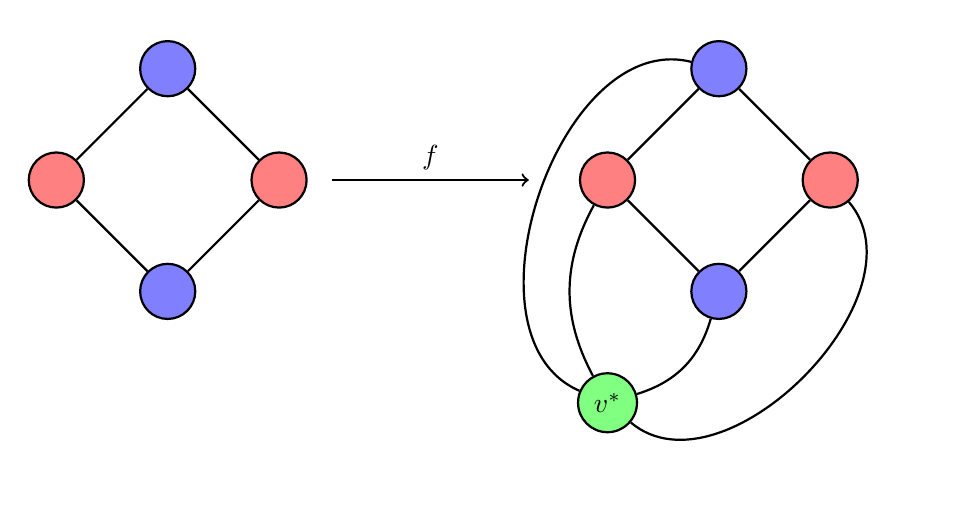
\begin{tikzpicture}[node distance={20mm}, thick,
             main/.style = {draw, circle, minimum size=0.7cm}]
            % Nodi grafo 1
            \node[main, fill = red!50] (1) {};
            \node[main, fill = blue!50] (2) [above right of=1] {};
            \node[main, fill = red!50] (3) [below right of=2] {};
            \node[main, fill = blue!50] (4) [below left of=3] {};

            \draw[<-] (6,0) -- (3.5,0) node[midway,above] {$f$};

            % Nodi grafo 2 identico a destra 
            \node[main, fill = red!50] (5) [right of=1, xshift=5cm] {};
            \node[main, fill = blue!50] (6) [above right of=5] {};
            \node[main, fill = red!50] (7) [below right of=6] {};
            \node[main, fill = blue!50] (8) [below left of=7] {};
            \node[main, fill = green!50] (9) [below left of=8] {$v^*$};

            % Archi
            \draw (1) -- (2);
            \draw (2) -- (3);
            \draw (3) -- (4);
            \draw (4) -- (1);

            \draw (5) -- (6);
            \draw (6) -- (7);
            \draw (7) -- (8);
            \draw (8) -- (5);
            \draw[bend left = 1cm] (8) to (9);
            \draw[bend left = 3cm] (7) to (9);
            \draw[bend right = 3cm] (6) to (9);
            \draw[bend right = 1cm] (5) to (9);
        \end{tikzpicture}
    \end{figure}
    L'idea è quella di aggiungere un vertice $v^*$ al grafo $\mathcal{G}$, e collegare $v^*$ a tutti i vertici
    di $\mathcal{G}$, in modo tale che $v^*$ abbia un colore diverso da tutti gli altri vertici.
    Per costruire la funzione $f$ possiamo procedere come segue:
    \begin{itemize}
        \item Dato un grafo $\mathcal{G}$, aggiungiamo un vertice $v^*$ al grafo $\mathcal{G}$.
        \item Colleghiamo $v^*$ a tutti i vertici di $\mathcal{G}$.
        \item Assegnamo a $v^*$ un colore diverso da tutti gli altri vertici, ovvero il colore $k+1$.
    \end{itemize}
    Se $\mathcal{G}$ è \texttt{k-colorabile}, allora esiste una colorazione $c$ tale che per ogni arco
    $(u,v) \in E$ si ha $c(u) \neq c(v)$. Se aggiungiamo un vertice $v^*$ al grafo $\mathcal{G}$, e lo colleghiamo
    a tutti i vertici di $\mathcal{G}$, allora $v^*$ deve avere un colore diverso da tutti gli altri vertici, ovvero
    il colore $k+1$. Quindi, se $\mathcal{G}$ è \texttt{k-colorabile}, allora $\mathcal{G'}$ è \texttt{(k+1)-colorabile}.
    
    Se $\mathcal{G}'$ è \texttt{(k+1)-colorabile} senza perdita di generalità diciamo che il colore di $v^*$ è $k+1$.
    Poiché per ogni $v$, $c(v) \neq k+1$, $c(v) \in \{1,\dots,k\}$ e quindi $c(v) \neq c(v^*)$, ovvero tutti i vertici $v$ hanno un colore diverso
    da $v^*$. Quindi, se $\mathcal{G'}$ è \texttt{(k+1)-colorabile},
    allora $\mathcal{G}$ è \texttt{k-colorabile}.
\section{Problemi \texttt{NP}-completi}
I problemi \texttt{NP}-completi sono una classe di problemi che sono problemi in \texttt{NP} e se uno 
di questi problemi è in \texttt{P}, allora tutti i problemi in \texttt{NP} sono in \texttt{P}, 
ovvero $\texttt{P} = \texttt{NP}$. Se $\texttt{P} \neq \texttt{NP}$, allora nessun problema
\texttt{NP}-completo è in \texttt{P}.
\begin{figure}[H]
    \centering
    \begin{tikzpicture}[set/.style={draw, circle, inner sep=0pt, align=center}]
        \node[set, fill=gray!40, text width=2.5cm] (P) at (0,0) {Problemi \texttt{P}};
        \node[set, fill=gray!40, text width=2.5cm] (NP) at (3,0) {\texttt{NP}-Completi};
        \begin{pgfonlayer}{background}
            \node[fill=gray!20, fit=(P) (NP), draw, rounded corners=0.5cm, inner
            sep=0.5cm, label={above: Problemi \texttt{NP}}] {};
        \end{pgfonlayer}
    \end{tikzpicture}
\end{figure}
Supponiamo che esista un problema $\mathbb{B}\in \texttt{NP}$ tale che per ogni problema $\mathbb{A}$ in \texttt{NP},
esiste una riduzione polinomiale da $\mathbb{A}$ a $\mathbb{B}$. 
Quindi se $\mathbb{B}$ è in \texttt{P}, allora $\mathbb{A}$ è in \texttt{P} allora 
per ogni problema $\mathbb{A}$ in \texttt{NP} esiste una riduzione polinomiale da
$\mathbb{A}$ a $\mathbb{B}$ e quindi $\mathbb{A}$ è in \texttt{P}.
Per contrapposizione, se $\texttt{P} \neq \texttt{NP}$,
allora $\mathbb{B}$ non è in \texttt{P} e quindi $\mathbb{A}$ non è in \texttt{P}.

Diciamo che $\mathbb{B}$ è \texttt{NP}-completo se $\mathbb{B}$ è in \texttt{NP} e
per ogni problema $\mathbb{A}$ in \texttt{NP}, $\mathbb{A}$ è riducibile a $\mathbb{B}$ in tempo polinomiale, 
ovvero $\mathbb{A} \leq_p \mathbb{B}$. 

\begin{tcolorbox}
    Un problema $\mathbb{B}$ è \texttt{NP}-completo se $\mathbb{B}$ è in \texttt{NP}
    e $\mathbb{B}$ è \texttt{NP}-hard.
\end{tcolorbox}

Un problema $\texttt{NP}$-completo deve essere un problema rappresentativo di tutti
i problemi in \texttt{NP}, deve essere quindi codificabile in modo tale che tutti i problemi
in \texttt{NP} siano riducibili a esso.

\subsection{Soddisfacibilità booleana}
Il problema della soddisfacibilità booleana è il problema di determinare se una formula booleana
è soddisfacibile, ovvero se esiste un assegnamento di valori di verità alle variabili della formula
che rende la formula vera. L'input al problema è una formula booleana in forma normale congiuntiva
(\texttt{CNF}) $\phi$ e l'output è \texttt{yes} se e solo se esiste un assegnamento di valori di verità
alle variabili della formula che rende la formula vera.

Una \textbf{formula booleana in forma normale congiuntiva (\texttt{CNF})} è definita come una
congiunzione di clausole. Formalmente, sia $\phi(x_1, \dots, x_n)$ una formula booleana
che dipende dalle variabili booleane $x_1, \dots, x_n$. Questa formula può essere espressa
come segue:
\[
\phi(x_1, \dots, x_n) = C^{(1)} \land C^{(2)} \land \dots \land C^{(m)}
\]
dove $m$ è il numero totale di clausole nella formula, e ogni clausola $C^{(i)}$ è definita
come una disgiunzione di uno o più letterali:
\[
C^{(i)} = l_1^{(i)} \lor l_2^{(i)} \lor \dots \lor l_{k_i}^{(i)}
\]
In questa definizione, $k_i$ rappresenta il numero di letterali nella $i$-esima clausola
$C^{(i)}$, e ogni letterale $l_j^{(i)}$ può essere una variabile booleana $x_t$ o la sua
negazione $\overline{x_t}$, per qualche $t \in \{1, \dots, n\}$. In altre parole, ogni letterale
è definito come:
\[
l_j^{(i)} \in \{x_1, \overline{x_1}, x_2, \overline{x_2}, \dots, x_n, \overline{x_n}\}
\]

Questa struttura garantisce che la formula $\phi$ sia una congiunzione di clausole, dove
ogni clausola è una disgiunzione di letterali, e ogni letterale è una variabile booleana
o la sua negazione.

Una formula \texttt{CNF} è quindi una funzione di $n$ variabili booleane che
restituisce un valore booleano. Un assegnamento $a$ di valori di verità alle
variabili della formula è una funzione $a: \{a_1, \dots, a_n\} \to \{0, 1\}$
che assegna un valore di verità a ciascuna variabile della formula. Un
assegnamento $a$ è detto \textbf{soddisfacente} per la formula $\phi$
se e solo se $\phi(a_1, a_2, \dots, a_n) = \texttt{true}$.
\subsubsection{Esempio}
Consideriamo la seguente formula booleana in forma normale congiuntiva:

\[
\phi(x_1, x_2, x_3, x_4) = (x_1 \lor x_2 \lor x_3 \lor \overline{x_4}) \land 
(\overline{x_1} \lor \overline{x_2}) \land (x_1 \lor x_2 \lor x_3 \lor \overline{x_4})
\]
Un assegnamento $a: \{a_1, a_2, a_3, a_4\} \to \{0, 1\}$ può essere il seguente:
\[
a = \{\texttt{true}, \texttt{false}, \texttt{true}, \texttt{true}\}
\]
Risolvendo la formula con l'assegnamento $a$ otteniamo:
\[
\phi(a_1, a_2, a_3, a_4) = \texttt{true} \land \texttt{true} \land \texttt{true} = \texttt{true}
\]
Quindi l'assegnamento $a$ soddisfa la formula $\phi$.

\subsubsection{Riduzione di \texttt{SAT} a \texttt{k-col}}
Prima di dimostrare che \texttt{SAT} è un problema \texttt{NP}-completo, dimostriamo
che \texttt{SAT} si riduce a \texttt{k-col}. L'obiettivo è mostrare che problemi molto 
diversi, come il problema di decisione su grafi, hanno una codifica in un problema 
di tipo logico come \texttt{SAT}.
\begin{tcolorbox}
    Dato un grafo $\mathcal{G}$, istanza di \texttt{k-col}, possiamo costruire in 
    tempo polinomiale una formula booleana $\phi_\mathcal{G}$ in forma normale congiuntiva
    tale che $\mathcal{G}$ è \texttt{k-col} se e solo se $\phi_\mathcal{G}$ è soddisfacibile.
\end{tcolorbox}
La misura del grafo $\mathcal{G}$ è definita come il numero di archi e nodi del grafo.
\[
    |\mathcal{G}=(V, E)| = |V| + |E|  
\]
Per una formula $\phi_\mathcal{G}$ in forma normale congiuntiva, la misura è il numero
    di letterali.

    Le variabili in $\phi_\mathcal{G}$ sono:
    \[
        x_1^{v_1}, x_2^{v_1}, \dots, x_k^{v_1}, x_1^{v_2},
        x_2^{v_2}, \dots, x_k^{v_2}, \dots, x_1^{v_n}, x_2^{v_n}, \dots, x_k^{v_n}
    \]
    Ovvero sia, per ogni vertice $v \in V$ abbiamo $k$ variabili $x_1^v, x_2^v, \dots, x_k^v$.
    
    Per ogni vertice $v \in V$ e per ogni colore $i \in \{1, \dots, k\}$, definiamo 
    la seguente clausola:
    \[
        C^{(v)} = x_1^v \lor x_2^v \lor \dots \lor x_k^v
    \]
    Ovvero, l'\texttt{OR} di tutte le variabili associate al vertice $v$, per ogni colore $i$,
    codificando il fatto che ad ogni vertice deve essere associato un colore. Con questa prospettiva
    almeno una delle variabili $x_1^v, x_2^v, \dots, x_k^v$ deve essere vera, e quindi almeno 
    un colore deve essere associato al vertice $v$.
    Non basta però dire che un colore deve essere associato ad ogni vertice, ma bisogna anche
    garantire che un vertice non possa avere due colori diversi. Per fare ciò, uno una nuova 
    clausola associata al vertice, ovvero su tutte le coppie possibili di colori 
    distinti, non vogliamo che al vertice $v$ siano associati entrambi i colori.
    \[
      D^{(v)} = \bigwedge_{1 \leq i < j \leq k} (\overline{x_i^v} \lor \overline{x_j^v})
    \]
    Se fosse vero, per esempio, che $x_1^v$ e $x_2^v$ sono entrambi veri, allora la clausola
    $D^{(v)}$ sarebbe falsa, e quindi la formula $\phi_\mathcal{G}$ sarebbe falsa. Questo
    garantisce che ad ogni vertice sia associato un solo colore.

    Questo non garantisce una colorazione propria, ovvero che vertici adiacenti abbiano colori
    diversi. Per fare ciò, per ogni arco $e = (u, v) \in E$, aggiungiamo la seguente clausola:
    \[
        E^{(e)} = \bigwedge_{1 \leq i \leq k} (\overline{x_i^u} \lor \overline{x_i^v})
    \]
    Se fosse vero che $x_i^u$ e $x_i^v$ sono entrambi veri, allora la clausola $E^{(e)}$ sarebbe
    falsa, e quindi la formula $\phi_\mathcal{G}$ sarebbe falsa. Questo garantisce che vertici
    adiacenti abbiano colori diversi.

    Definiamo ora la formula $\phi_\mathcal{G}$ come:
    \begin{equation}
        \label{eq:phi}
        \phi_\mathcal{G} = \bigwedge_{v \in V} \left(C^{(v)} \land D^{(v)}\right) \land \bigwedge_{e \in E} E^{(e)}
    \end{equation}
La dimensione della formula è:
\[
    |\phi_\mathcal{G}| = |V| \cdot \left(k + \left(\frac{k}{2}\right) \cdot 2 \right) 
    + |E| \cdot k \cdot 2 = O(|V| \cdot k + |E| \cdot k) = O( k \cdot (|V| + |E|) )
\]
Quindi polinomiale nella taglia del grafo.
\subsubsection{Esempio}
Consideriamo il seguente grafo $\mathcal{G}$ e una \texttt{2-col}:

\begin{minipage}{0.5\textwidth}
    \begin{figure}[H]
        \centering
        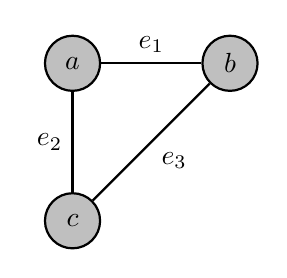
\begin{tikzpicture}[node distance={20mm}, thick,
            main/.style = {draw, circle, minimum size=0.7cm}]

           \node[main, fill = gray!50] (1) {$a$};
           \node[main, fill = gray!50] (2) [below of=1] {$c$};
           \node[main, fill = gray!50] (3) [right of=1] {$b$};

            %archi con etichetta 
            \draw (1) -- (3) node[midway, above] {$e_1$};
            \draw (1) -- (2) node[midway, left] {$e_2$};
            \draw (2) -- (3) node[midway, below right] {$e_3$};
        \end{tikzpicture}
    \end{figure}
\end{minipage}
\begin{minipage}{0.5\textwidth}
    \begin{align*}
        V &= \{a, b, c\} \\
        E &= \{(a, b), (a, c), (b, c)\}
    \end{align*}
\end{minipage}

Quindi definiamo le clausole:
\[
  C^{(a)} = x_1^a \lor x_2^a
 \qquad
  D^{(a)} = (\overline{x_1^a} \lor \overline{x_2^a})
\]
\[
  C^{(b)} = x_1^b \lor x_2^b
  \qquad
  D^{(b)} = (\overline{x_1^b} \lor \overline{x_2^b})
\]
\[
  C^{(c)} = x_1^c \lor x_2^c
  \qquad
  D^{(c)} = (\overline{x_1^c} \lor \overline{x_2^c})
\]
\[ 
    E^{(e_1)} = (\overline{x_1^a} \lor \overline{x_1^b}) \land (\overline{x_2^a} \lor \overline{x_2^b})
\]
\[ 
    E^{(e_2)} = (\overline{x_1^a} \lor \overline{x_1^c}) \land (\overline{x_2^a} \lor \overline{x_2^c})
\]
\[ 
    E^{(e_3)} = (\overline{x_1^b} \lor \overline{x_1^c}) \land (\overline{x_2^b} \lor \overline{x_2^c})
\]

Quindi la formula $\phi_\mathcal{G}$ è:
\[
    \phi_\mathcal{G} = C^{(a)} \land D^{(a)} \land C^{(b)} \land D^{(b)} \land C^{(c)} \land D^{(c)} \land E^{(e_1)} \land E^{(e_2)} \land E^{(e_3)}
\]

Dimostriamo che \texttt{k-col} si riduce polinomialmente a \texttt{SAT}.
\begin{theorem}
    $\texttt{k-col} \leq_p \texttt{SAT}$
\end{theorem}
\begin{proof} Dimostriamo entrambi i versi dell'implicazione.
    
    $(\Rightarrow)$

    
    Dimostriamo prima che se $\mathcal{G}$ è $k$-colorabile, allora $\phi_\mathcal{G}$ è
    soddisfacibile.

    Sia $\{c(v) \mid v \in V\}$ una colorazione propria di $\mathcal{G}$, ossia, per ogni
    arco $e=(u, v) \in E$, vale che $c(u) \neq c(v)$ e $c(v) \in \{1, \ldots, k\}$. Definiamo
    l'assegnamento $a_j^{v_i}$ come segue: 
    \[
    a_j^{v_i} =
    \begin{cases}
        \texttt{true} & \text{se } c(v_i) = j, \\
        \texttt{false} & \text{altrimenti}.
    \end{cases}
    \]
    Dimostriamo ora che questo assegnamento soddisfa tutte le clausole di $\phi_\mathcal{G}$.
    \begin{enumerate}
        \item Per la clausola $C^{(v)}$, che assicura che ogni vertice $v$ riceva almeno un colore:
        \begin{align*}
            \exists c(v_i) = j & \implies a_j^{v_i} = \texttt{true} \\
            & \implies C^{(v)}(a) = \texttt{true}.
        \end{align*}
        
        \item Per la clausola $D^{(v)}$, che previene che un vertice $v$ abbia più di un colore:
        \begin{align*}
            \forall i \neq j, \, a_i^{v} = \texttt{false} \lor a_j^{v} = \texttt{false} & \implies
            D^{(v)}(a) = \texttt{true}.
        \end{align*}
        
        \item Per la clausola $E^{(e)}$, che assicura che due vertici adiacenti $u$ e $v$ non
        abbiano lo stesso colore:
        \begin{align*}
            c(u) \neq c(v) & \implies \forall i, \, a_i^{u} = \texttt{false} \lor a_i^{v} =
            \texttt{false} \\
            & \implies E^{(e)}(a) = \texttt{true}.
        \end{align*}
    \end{enumerate}
    Questo dimostra che se $\mathcal{G}$ è $k$-colorabile, allora esiste un assegnamento
    di verità che soddisfa $\phi_\mathcal{G}$, ovvero la formula $\phi_\mathcal{G}$ è soddisfacibile.

    $(\Leftarrow)$

    Ora dimostriamo che se $\phi_\mathcal{G}$ è soddisfacibile, allora $\mathcal{G}$ è $k$-colorabile.

    Assumiamo che esista un assegnamento di verità $a$ che soddisfa $\phi_\mathcal{G}$ e mostriamo 
    che $\mathcal{G}$ è $k$-colorabile. Questa parte di dimostrazione serve ad evitare che 
    la formula $\phi_\mathcal{G}$ possa essere soddisfatta da un assegnamento che non rappresenti
    una colorazione propria di $\mathcal{G}$.

    Esiste l'assegnamento $a = (a_1^{v_1}, \ldots, a_k^{v_1}, \ldots, a_1^{v_n}, \ldots, a_k^{v_n})$ 
    tale che $\phi_\mathcal{G}(a) = \texttt{true}$. Mostriamo che da questo assegnamento possiamo
    costruire una colorazione propria di $\mathcal{G}$.
    Per farlo, definiamo una colorazione per $\mathcal{G}$ basata su $a$ come segue:
    \[
        \forall v \in V, \quad c(v) = i \iff a_i^v = \texttt{true}.
    \]
    \begin{enumerate}
        \item Ogni vertice $v$ è colorato con un solo colore. Possiamo esprimere questa condizione come segue:
        \begin{align*}
            \phi(a) = \texttt{true} & \implies C^{(v)}(a) = \texttt{true} \\
            & \implies \exists i \in \{1, \ldots, k\} \text{ tale che } a_i^v = \texttt{vero} \\
            & \implies c(v) = i.
        \end{align*}
        \item Ogni vertice $v$ è colorato con un solo colore. Possiamo esprimere questa
        condizione come segue:
        \begin{align*}
            \phi(a) = \texttt{true} & \implies D^{(v)}(a) = \texttt{true} \\
            & \implies \nexists i, j \in \{1, \ldots, k\}
            \text{ tali che } a_i^v = a_j^v = \texttt{true} \\
            & \implies \exists i \in \{1, \ldots, k\} \text{ tale che } c(v) = i.
        \end{align*}
        perché se esistessero due colori $i, j$ tali che $a_i^v = a_j^v = \texttt{true}$, allora
        $C^{(v)}(a) = \texttt{false}$, che è assurdo.
        \item Dimostriamo che la colorazione è propria, ossia che ogni arco non è monocromatico,
        ossia che per ogni arco $e = (u, v) \in E$, $c(u) \neq c(v)$. Possiamo esprimere questa
        condizione come segue:
        \begin{align*}
            \phi(a) = \texttt{true} & \implies E^{(e)}(a) = \texttt{true} \\
            & \implies \nexists i \in \{1, \ldots, k\} \text{ tale che } a_i^u = a_i^v = \texttt{true} \\
            & \implies \nexists i \in \{1, \ldots, k\} \text{ tale che } c(u) = c(v) \\
            & \implies c(u) \neq c(v).
        \end{align*}
    \end{enumerate}

    Questo dimostra che se $\phi_\mathcal{G}$ è soddisfacibile, allora $\mathcal{G}$ è
    $k$-colorabile.

    Abbiamo dimostrato che $\mathcal{G}$ è $k$-colorabile se e solo se $\phi_\mathcal{G}$ è
    soddisfacibile. 
\end{proof}
Questo teorema dimostra che la difficoltà di risolvere il problema della colorazione di un grafo
è equivalente alla difficoltà di risolvere il problema della soddisfacibilità di una formula
booleana. 

\subsection{\texttt{Circuit-SAT}}
Il problema \texttt{Circuit-SAT} è un problema di soddisfacibilità di una formula booleana
particolare, in cui la formula è rappresentata da un circuito logico. Un circuito logico è una
rappresentazione di una formula booleana in cui le porte logiche sono connesse tra loro da
cavi. Ogni porta logica è rappresentata da un nodo del circuito, mentre i cavi sono rappresentati
dagli archi del circuito.

L'input del problema \texttt{Circuit-SAT} è un circuito logico $\mathcal{C}$ e
l'output è \texttt{yes} se e solo se il circuito $\mathcal{C}$ è soddisfacibile.

Si tratta di un grafo aciclico diretto (\texttt{DAG}) in cui i nodi
interni sono porte logiche e i nodi di input sono costituiti da variabili booleane.
\begin{figure}[H]
    \centering
    \begin{tikzpicture}[circuit logic US, every circuit symbol/.style={thick}]
        % Inputs
        \node (x1) at (0, 0) {$x_1$};
        \node (x2) at (0, -1) {$x_2$};
        \node (x3) at (0, -2) {$x_3$};
        \node (x4) at (0, -3) {$x_4$};
        \node (x5) at (0, -4) {$x_5$};

        % Logic gates
        \node[and gate, draw, logic gate inputs=nn] at (2, -0.5) (p1) {};
        \node[or gate, draw, logic gate inputs=nn] at (2, -2.5) (p2) {};
        \node[not gate, draw] at (2, -4) (p3) {};

        \node[and gate, draw, logic gate inputs=nn] at (4, -1.5) (p4) {};

        \node[and gate, draw] at (6, -2.5) (p6) {};

        % Output
        \node (y) at (8, -2.5) {$y$};

        % Connections
        \draw (x1.east) -- ([xshift=0.2cm]x1.east) |- (p1.input 1);
        \draw (x2.east) -- ([xshift=0.2cm]x2.east) |- (p1.input 2);
        \draw (x3.east) -- ([xshift=0.2cm]x3.east) |- (p2.input 1);
        \draw (x4.east) -- ([xshift=0.2cm]x4.east) |- (p2.input 2);
        \draw (x5.east) -- (p3.input);
        \draw (p1.output) -- ([xshift=0.2cm]p1.output) |- (p4.input 1);
        \draw (p2.output) -- ([xshift=0.2cm]p2.output) |- (p4.input 2);
        \draw (p4.output) -- ([xshift=0.2cm]p4.output) |- (p6.input 1);
        \draw (p3.output) -- ([xshift=0.2cm]p3.output) |- (p6.input 2);
        \draw (p6.output) -- (y.west);
    \end{tikzpicture}
    \caption{Esempio di circuito logico}
\end{figure}
Ogni vertice del circuito logico ha associato l'operatore booleano \texttt{AND},
\texttt{OR} o \texttt{NOT}. In particolare l'operatore \texttt{NOT} è associato
a nodi con \textit{in-degree} $1$, mentre gli operatori \texttt{AND} e \texttt{OR} sono associati
a nodi con \textit{in-degree} $2$.
I vertici con \textit{in-degree} $0$ sono detti \textit{input}, mentre i vertici
con \textit{out-degree} $0$ sono detti \textit{output}.

Dato un assegnamento booleano $a$ delle variabili di input,
possiamo valutare il circuito logico $\mathcal{C}$ assegnando ad ogni nodo
il valore booleano corrispondente all'operatore associato al nodo e ai valori
booleani dei nodi di input. In questo modo possiamo valutare il circuito logico
come una formula booleana.

\subsection{\texttt{NP}-completezza di \texttt{SAT}}

\begin{theorem}[di Cook-Levin]
    Il problema \texttt{SAT} è \texttt{NP}-completo.
\end{theorem}
Per dimostrare il seguente teorema utilizziamo il seguente lemma.
\begin{lemma}
    \label{lemma:np-completeness}
    Per ogni problema in $\mathbb{B} \in \texttt{P}$ e per ogni $n \in \mathbb{N}$,
    esiste un circuito booleano $\mathcal{C}_n$ tale che per ogni $x \in \mathcal{I}(\mathbb{B})$
    tale che $|x| = n$, $\mathbb{B}(x) = 1$ se e solo se $\mathcal{C}_n(x) = 1$, ovvero
    \[
        \texttt{C}_n(x) = \mathbb{B}(x)  
    \]
    Inoltre $\mathcal{C}_n$ ha dimensione polinomiale rispetto a $n$.
\end{lemma}
\begin{proof}
    Per dimostrare che \texttt{SAT} è \texttt{NP}-completo, dobbiamo dimostrare che
    \begin{enumerate}
        \item \texttt{SAT} è in \texttt{NP}.

            Sappiamo che \texttt{SAT} è in \texttt{NP} in quanto
            possiamo verificare in tempo polinomiale una soluzione proposta per il problema.
        \item $\texttt{Circuit-SAT}$ è \texttt{NP}-completo.
            
        Dimostrare che $\texttt{Circuit-SAT}$ è \texttt{NP}-completo equivale a dimostrare
            che \texttt{Circuit-SAT} appartiene a \texttt{NP}
            e per ogni problema in \texttt{NP} esiste una riduzione polinomiale da esso a
            $\texttt{Circuit-SAT}$.
            \begin{itemize}
                \item Dimostriamo che \texttt{Circuit-SAT} appartiene a \texttt{NP}. Dato un circuito logico
                    $\mathcal{C}$ e un assegnamento booleano $a$ delle variabili di input, possiamo valutare
                    il circuito logico $\mathcal{C}$ assegnando ad ogni nodo il valore booleano corrispondente
                    all'operatore associato al nodo e ai valori booleani dei nodi di input. In questo modo
                    possiamo valutare il circuito logico come una formula booleana. Se la formula booleana
                    è soddisfacibile, allora il circuito logico $\mathcal{C}$ è soddisfacibile.
                \item Sfruttiamo il lemma \ref{lemma:np-completeness} per dimostrare che $\texttt{Circuit-SAT}$ è
                    \texttt{NP}-completo.

                    Per ogni problema \( \mathbb{A} \) appartenente alla classe \texttt{NP}, possiamo
                    affermare
                    che \( \mathbb{A} \) è riducibile a \texttt{Circuit-SAT}. Questa riduzione comporta la
                    definizione di una trasformazione che, fissato un input \( x \) appartenente all'insieme
                    delle istanze \( \mathcal{I}(\mathbb{A}) \) di \( \mathbb{A} \), genera un circuito
                    booleano \( \mathcal{C}^{\mathbb{A}}_x \) tale che \( \mathbb{A}(x) = 1 \) se e solo
                    se \( \mathcal{C}^{\mathbb{A}}_x \) è soddisfacibile.

                    Essendo \( \mathbb{A} \) un problema in \texttt{NP}, esiste un verificatore
                    polinomiale \( B(x,y) \) che determina se \( y \) è una soluzione corretta per
                    l'input \( x \) fissato, per ogni \( x \) in \( \mathcal{I}(\mathbb{A}) \). In altre parole:

                    \[
                    \mathbb{A}(x) = \texttt{yes} \iff \exists y \in \{0,1\}^{|x|^c} : B(x,y) = \texttt{yes}
                    \]

                    dove \( y \) è una stringa di lunghezza polinomiale in \( |x| \) e \( c \) è una
                    costante.

                    Il calcolo di \( B(x,y) \) appartiene alla classe \texttt{P}, il che implica che,
                    fissato l'input \( x \), esiste un circuito booleano \( \mathcal{C}^{\mathbb{A}}_x \)
                    di dimensione polinomiale che, per ogni assegnazione di \( y \) di lunghezza \( n \),
                    soddisfa la relazione \( \mathcal{C}^{\mathbb{A}}_x(y) = B(x,y) \).

                    Quindi, \( \mathcal{C}^{\mathbb{A}}_x \) rappresenta un circuito booleano che può essere
                    costruito in tempo polinomiale e che codifica il problema \( \mathbb{A} \) per
                    un'istanza specifica \( x \) fissata.

                    \[
                    x \in \mathcal{I}(\mathbb{A}) \qquad \mathbb{A}(x) = 1 \iff \exists y \quad t.c.
                     \quad B(x,y) = 1 \iff \exists y \quad t.c. \quad \mathcal{C}^{\mathbb{A}}_x(y) = 1
                    \]

                    Abbiamo così dimostrato che, per ogni problema in \texttt{NP}, esiste una riduzione
                    polinomiale a \texttt{Circuit-SAT}, con l'input \( x \) fissato durante la
                    trasformazione.
            \end{itemize}
        \item $\texttt{Circuit-SAT} \leq_p \texttt{SAT}$.
            
            Dato il seguente circuito booleano $\mathcal{C}$:
            \begin{figure}[H]
                \centering
                \begin{tikzpicture}[circuit logic US, every circuit symbol/.style={thick}]
                    % Inputs
                    \node (x1) at (0, 0) {$x_1$};
                    \node (x2) at (0, 1) {$x_2$};
                    \node (x3) at (0, 2) {$x_3$};
            
                    % Logic gates
                    \node[or gate, draw, logic gate inputs=nn] at (2, 0.5) (p1) {};
                    \node[not gate, draw] at (2, 2) (p2) {};
                    \node[and gate, draw] at (4, 1) (p3) {};
            
                    % Output
                    \node (y) at (6, 1) {$y_3$};
            
                    % Connections
                    \draw (x1.east) -- ([xshift=0.2cm]x1.east) |- (p1.input 2);
                    \draw (x2.east) -- ([xshift=0.2cm]x2.east) |- (p1.input 1);
                    \draw (x3.east) -- ([xshift=0.2cm]x3.east) |- (p2.input);

                    \draw (p1.output) -- ([xshift=0.2cm]p1.output) |- node[midway, below right] {$y_2$} (p3.input 2);
                    \draw (p2.output) -- ([xshift=0.2cm]p2.output) |- node[midway, above right] {$y_1$} (p3.input 1);
                    
                    \draw (p3.output) -- (y.west);
                \end{tikzpicture}
                \caption{Circuito booleano $\mathcal{C}$}
            \end{figure}
            Vogliamo trasformare il circuito booleano $\mathcal{C}$ in una
            formula booleana $\phi$ in forma normale congiuntiva, in una 
            riduzione polinomiale tale che:
            \[
                \mathcal{C}(x) = 1 \iff \exists x' \quad t.c. \quad \phi(x') = 1
            \]
            Per farlo prendiamo tutti gli output del circuito e gli assegnamo 
            una variabile, in questo caso $y_i$ con $i \in \{1, 2, 3\}$ e le fissiamo 
            rispetto alle variabili di input. In questo caso abbiamo che:
            \[
                y_1 = \overline{x_3} \quad y_2 = x_1 \lor x_2 \quad y_3 = y_1 \land y_2
            \]
            Non sono quindi libere nella formula $\phi$ le variabili $y_i$ ma 
            sono fissate rispetto alle variabili di input. Inoltre $y_3$ è dovrà 
            essere a $1$ per far si che il circuito sia soddisfacibile.

            La formula $\phi$ sarà quindi:
            \[
                \phi(x_1, x_2, x_3, y_1, y_2, y_3) 
                = \big[ (x_1 \lor x_2) = y_1 \big] \land 
                \big[ \overline{x_3} = y_2 \big] \land 
                \big[ y_1 \land y_2 = y_3 \big] \land
                y_3
            \]
            Quindi abbiamo che:
            \[
                \exists x \quad t.c. \quad \mathcal{C}(x) = 1
                \iff \exists x,y \quad t.c. \quad \phi(x, y) = 1
            \]
            Per trasformare la formula $\phi$ in una formula in forma normale
            congiuntiva possiamo utilizzare le equivalenze logiche.

            Passiamo quindi da un circuito che ha un numero di input $n$ ad una 
            formula che ha un numero di variabili polinomiale in $n$, da qui 
            otteniamo una formula in forma normale congiuntiva (\textit{applicando 
            le equivalenze logiche}) che ha un numero di clausole polinomiale in $n$ 
            che è soddisfacibile se e solo se il circuito è soddisfacibile.
    \end{enumerate}
    Sappiamo che per ogni $\mathbb{A} \in \texttt{NP}, \mathbb{A}
    \leq_p \texttt{Circuit-SAT} \leq_p \texttt{SAT}$, quindi abbiamo 
    $\texttt{SAT} \in \texttt{NP}-completo$.
\end{proof}
\subsection{Formule \texttt{K-CNF}}
Una formula \texttt{K-CNF} è una formula in forma normale congiuntiva 
dove ogni clausola ha al più $k$ letterali.

Per esempio la formula:
\[
    \phi = (x_1 \lor x_2 \lor x_3) \land (x_1 \lor x_2 \lor x_4) \land
    (\overline{x_1} \lor x_2 \lor x_3 \lor x_4 \lor x_5)
\]
è una formula \texttt{5-CNF}.

\begin{theorem}
    \texttt{3-SAT} è \texttt{NP-completo}.
\end{theorem}

\begin{proof}
    Per dimostrare che \texttt{3-SAT} è \texttt{NP-completo} dobbiamo dimostrare che:
    \begin{enumerate}
        \item \texttt{3-SAT} è in \texttt{NP}.
        \item \texttt{3-SAT} è \texttt{NP-hard}.
    \end{enumerate}

    Banalmente, \texttt{3-SAT} è in \texttt{NP} in quanto possiamo verificare in tempo
    polinomiale se un'assegnazione di valori alle variabili soddisfa la formula.

    Dimostriamo ora che \texttt{3-SAT} è \texttt{NP-hard} dimostrando che \texttt{SAT}
    si riduce in tempo polinomiale a \texttt{3-SAT}. Questo possiamo farlo, in quanto
    conosciamo che \texttt{SAT} è \texttt{NP}-completo e quindi possiamo ridurre
    \texttt{SAT} a \texttt{3-SAT}. Per farlo, sfruttiamo una trasformazione clausola per
    clausola, trasformando una clausola con $k$ letterali in una serie di clausole in
    \texttt{3-CNF} che possono essere soddisfatte se e solo se la clausola originale è
    soddisfacibile. Questa trasformazione garantisce che la formula risultante sia in
    \texttt{3-CNF} e abbia una lunghezza polinomiale rispetto alla formula originale.

    Supponiamo che $C$ sia una clausola:
    \[
        C = (l_1 \lor l_2 \lor l_3 \lor \ldots \lor l_k)
    \]
    dove $k > 3$ e $l_i$ sono letterali che possono essere variabili booleane o le
    loro negazioni. Possiamo trasformare $C$ in una formula in forma normale congiuntiva
    a tre termini (\texttt{3-CNF}) introducendo una serie di variabili ausiliarie $z_i$.
    La trasformazione procede come segue:
    \[ 
        C' = (l_1 \lor l_2 \lor z_1) \land (\overline{z_1} \lor l_3 \lor z_2) \land \ldots
        \land (\overline{z_{k-3}} \lor l_{k-1} \lor l_k)
    \]
    In questa trasformazione, ogni nuova clausola contiene esattamente tre letterali,
    aderendo alla definizione di \texttt{3-CNF}. La formula risultante $C'$ consiste
    di $k-2$ clausole, poiché per ogni letterale in $C$ oltre ai primi tre, inseriamo
    una nuova clausola che utilizza una variabile ausiliaria introdotta. Ciò mantiene
    la struttura richiesta per una formula \texttt{3-CNF}, assicurando che ogni clausola
    abbia al massimo tre letterali.

    La trasformazione aggiunge un totale di $k-3$ variabili ausiliarie, poiché ogni nuova
    variabile ausiliaria $z_i$ è utilizzata per collegare le clausole tra loro in modo che
    la formula complessiva sia equivalente alla clausola originale $C$ in termini di
    soddisfacibilità.

    Perciò, la taglia della formula risultante è polinomiale rispetto alla taglia della
    formula originale, e la trasformazione può essere eseguita in tempo polinomiale.

    Mostriamo ora che se $C$ è soddisfacibile, allora $C'$ è soddisfacibile. Supponiamo
    che esista un assegnamento di valori alle variabili che soddisfa $C$.
    Dato che almeno uno dei letterali in $C$ è vero, possiamo assegnare valori
    alle variabili ausiliarie in modo da garantire che ogni clausola in $C'$ sia
    soddisfatta. Ad esempio, se $l_1$ è vero, allora la prima clausola di $C'$ è
    soddisfatta. Possiamo poi assegnare a ciascuna variabile ausiliaria $z_i$ un
    valore che assicuri la soddisfazione delle clausole successive, tenendo conto
    che ogni clausola contiene o una variabile ausiliaria o la sua negazione insieme
    a letterali di $C$. Pertanto,
    se $C$ è soddisfacibile, possiamo costruire un assegnamento che soddisfa anche $C'$.

    Mostriamo che se $C'$ è soddisfacibile, allora $C$ è soddisfacibile. Supponiamo che
    esista un assegnamento di valori alle variabili che soddisfa $C'$.
    Dato che $C'$ è soddisfacibile, almeno uno dei letterali in ogni clausola di $C'$
    deve essere vero.

    Quindi esiste un assegnamento $a_x$ e $a_z$ tale che $a_x$ e $a_z$ soddisfano $C'$.
    Supponiamo per assurdo che $a_x$ non soddisfi $C$. Quindi tutti i letterali $l_i$
    in $C'$ sono falsi.

    Avendo una clausola del tipo:
    \[
        C' = (\texttt{false} \lor \texttt{false} \lor z_1) 
        \land (\overline{z_1} \lor \texttt{false} \lor z_2) \land \ldots
        \land (\overline{z_{k-3}} \lor \texttt{false} \lor \texttt{false})
    \]
    La clausola non può essere soddisfatta, in quanto per soddisfare la prima 
    sottoclausola, $z_1$ deve essere vero, ma per soddisfare la seconda sottoclausola,
    $z_2$ deve essere vero e così via. Ma per soddisfare l'ultima sottoclausola,
    $z_{k-3}$ deve essere falso, il che è una contraddizione, poiché $z_{k-3}$ deve
    essere vero per soddisfare la penultima sottoclausola.
    Quindi $a_x$ deve soddisfare $C$ per soddisfare $C'$.

    Consideriamo il caso in cui $k < 3$.

    Data una formula in forma normale congiuntiva con clausole minori o uguali a tre
    letterali $\phi$, possiamo trasformarla in una formula in forma normale congiuntiva $\varphi$
    con clausole esattamente di tre letterali tale che $\phi$ sia soddisfacibile se e
    solo se $\varphi$ è soddisfacibile.

    Supponiamo che $\phi$ contenga una clausola $C$ con $k$ letterali, dove $k < 3$ 
    e dimostriamo che $C$ è soddisfacibile se e solo se $C'$ è soddisfacibile.

    Supponiamo che $C$ sia una clausola con un solo letterale:
    \[
        C = (l_1)
    \]
    La trasformazione procede come segue:
    \[
        C' = (l_1 \lor z_1 \lor z_2) \land (l_1 \lor
        \overline{z_1} \lor z_2) \land (l_1 \lor z_1 \lor \overline{z_2})
        \land (l_1 \lor \overline{z_1} \lor \overline{z_2})
    \]
    In questa trasformazione, ogni nuova clausola contiene esattamente tre letterali,
    aderendo alla definizione di \texttt{3-CNF}. Se $l_1$ è vero, allora tutte le
    clausole in $C'$ sono soddisfatte. Se $l_1$ è falso, allora almeno una delle
    clausole in $C'$ non è soddisfatta, garantendo che $C'$ sia soddisfacibile se e
    solo se $C$ è soddisfacibile.

    Supponiamo ora che $C$ contenga due letterali:
    \[
        C = (l_1 \lor l_2)
    \]
    La trasformazione procede come segue:
    \[
        C' = (l_1 \lor l_2 \lor z_1) \land (l_1 \lor l_2 \lor \overline{z_1})
    \]
    Se la formula originale è soddisfacibile, allora o $l_1$ o $l_2$ è vero, e
    quindi la clausola $C'$ è soddisfatta. Se $C$ non è soddisfacibile, allora
    $l_1$ e $l_2$ sono entrambi falsi, e quindi $C'$ non è soddisfacibile, poiché 
    non esiste alcun valore di verità per $z_1$ che possa rendere soddisfatta la
    clausola.

    Dimostriamo ora che se $C'$ è soddisfacibile, allora $C$ è soddisfacibile.
    Se $C'$ è soddisfacibile, allora esiste un assegnamento $a_x$ e $a_z$ tale che
    $a_x$ e $a_z$ soddisfano $C'$. Supponiamo per assurdo che $a_x$ non soddisfi $C$.
    
    Quindi nel caso in cui $C$ contenga un solo letterale, avrei:
    \[
        C' = (\texttt{false} \lor z_1 \lor z_2) \land
        (\texttt{false} \lor \overline{z_1} \lor z_2)
        \land (\texttt{false} \lor z_1 \lor \overline{z_2}) \land
        (\texttt{false} \lor \overline{z_1} \lor \overline{z_2})
    \]
    Disponendo di tutte le configurazioni possibili, non esiste un assegnamento
    che possa soddisfare $C'$, poiché almeno uno dei letterali deve essere vero
    per soddisfare la clausola. Quindi $a_x$ deve soddisfare $C$ per soddisfare
    $C'$. Il ragionamento può essere esteso a tutte le clausole con due letterali
    di $\phi$, dimostrando che se $C'$ è soddisfacibile, allora $C$ è soddisfacibile.
    Quindi abbiamo dimostrato che se $C'$ è soddisfacibile, allora $C$ è soddisfacibile.

    Nel caso in cui la clausola contenga tre letterali, allora $C$ è già in forma
    normale congiuntiva, e quindi $C$ è soddisfacibile se e solo se $C'$ è soddisfacibile.

    Perciò abbiamo dimostrato che \texttt{3-SAT} è \texttt{NP}-completo.
\end{proof}
\subsection{\texttt{NP}-completezza di \texttt{NAE-K-SAT}}
Introduciamo ora il problema \texttt{NAE-K-SAT} (\textit{Not-All-Equal \texttt{K-SAT}}).
L'istanza di un problema \texttt{NAE-K-SAT} è una formula in forma normale congiuntiva 
e l'output è \texttt{yes} se e solo se esiste un assegnamento di valori alle variabili 
che soddisfa la formula e in cui ogni clausola contiene almeno un letterale vero e almeno
un letterale falso.

Esiste quindi un assegnamento $a$ tale che per ogni clausola $C$ della formula, l'assegnamento 
$a$ pone almeno un letterale di $C$ a \texttt{true} e almeno un letterale di $C$ a \texttt{false}.

\subsubsection{Esempio}
Supponiamo di avere la seguente formula in forma normale congiuntiva:
\[
    \phi(x_1, x_2, x_3) = (x_1 \lor \overline{x_2} \lor x_3)
    \land (\overline{x_1} \lor \overline{x_2} \lor x_3)
\]
Un assegnamento del tipo $a = (x_1 = \texttt{true}, x_2 = \texttt{false}, x_3 = \texttt{true})$
non soddisfa la formula, in quanto la prima clausola è soddisfatta, ma la seconda clausola
non è soddisfatta. Un assegnamento del tipo $a = (x_1 = \texttt{false}, x_2 = \texttt{false},
x_3 = \texttt{true})$
soddisfa la formula, in quanto entrambe le clausole sono soddisfatte.

\begin{lemma}
    Data una formula in forma normale congiuntiva $\phi$, se $a=(a_1, \ldots, a_n)$
    \texttt{NAE} soddisfa $\phi$, allora anche l'assegnamento
    $a'=(\overline{a_1}, \ldots, \overline{a_n})$ \texttt{NAE}
    soddisfa $\phi$.
\end{lemma}

Dimostriamo ora che \texttt{NAE-K-SAT} è \texttt{NP-completo}, partendo dalla dimostrazione
che \texttt{NAE-3-SAT} è in \texttt{NP-completo}.
\begin{theorem}
    \texttt{NAE-3-SAT} è \texttt{NP-completo}.
\end{theorem}

\begin{proof}
Per dimostrare che \texttt{NAE-3-SAT} è \texttt{NP-completo}, dobbiamo mostrare che:
\begin{enumerate}
    \item \texttt{NAE-3-SAT} è in \texttt{NP}.
    \item \texttt{NAE-3-SAT} è \texttt{NP-hard}.
\end{enumerate}
\textbf{1. \texttt{NAE-3-SAT} è in \texttt{NP}:} È possibile verificare in tempo
polinomiale un dato assegnamento di verità per tutte le clausole, assicurando che
ogni clausola abbia almeno un letterale vero e uno falso.

\textbf{2. \texttt{NAE-3-SAT} è \texttt{NP-hard}:} Dimostriamo che \texttt{3-SAT}
si riduce in tempo polinomiale a \texttt{NAE-4-SAT}, che a sua volta si riduce
a \texttt{NAE-3-SAT}:
\[
  \texttt{3-SAT} \leq_p \texttt{NAE-4-SAT} \leq_p \texttt{NAE-3-SAT}
\]
\begin{itemize}
    \item \textbf{Riduzione da \texttt{3-SAT} a \texttt{NAE-4-SAT}:} Per ogni
    clausola $C$ in una formula \texttt{3-SAT}, aggiungiamo una variabile ausiliaria
    $z$ per formare la clausola $D = (C \lor z)$ nella formula \texttt{NAE-4-SAT}.
    
    La nuova formula \texttt{NAE-4-SAT}
    è soddisfacibile se e solo se la formula \texttt{3-SAT} originale è soddisfacibile.
        \begin{description}
            \item[$(\Rightarrow)$] Se $\varphi$ in \texttt{3-SAT} è soddisfacibile con
            un assegnamento $a = (a_1, \dots, a_n)$, allora l'assegnamento $b =
            (a_1, \dots, a_n, \texttt{false})$ soddisfa $\psi$ in \texttt{NAE-4-SAT}
            poiché l'aggiunta di $z = \texttt{false}$ non altera la soddisfacibilità
            di ogni clausola $D^{(i)}$.
            \item[$(\Leftarrow)$] Se $\psi$ in \texttt{NAE-4-SAT} è soddisfacibile
            con un assegnamento $b = (b_1, \dots, b_n, b_{n+1})$, possiamo ottenere
            un assegnamento per $\varphi$ in \texttt{3-SAT} ponendo $a = (b_1, \dots, b_n)$.
            Se $b_{n+1} = \texttt{true}$, invertiamo ogni valore di $b_1, \dots, b_n$
        per soddisfare $\phi$.
        \end{description}
    \item \textbf{Riduzione da \texttt{NAE-4-SAT} a \texttt{NAE-3-SAT}:} 
    L'obiettivo è mostrare che se una clausola $\psi$ di \texttt{NAE-4-SAT} è 
    soddisfacibile, allora esiste un assegnamento che soddisfa anche una clausola
    $\varphi$ di \texttt{NAE-3-SAT}.

    Supponiamo che la clausola $\psi$ in \texttt{NAE-4-SAT} sia nella forma:
    \[
        \psi = C^{(1)} \land C^{(2)} \land C^{(3)} \land C^{(4)}
    \]
    dove $C^{(i)}$ è una clausola con al più quattro letterali
    \[
        C^{(i)} = l_1^{(i)} \lor l_2^{(i)} \lor l_3^{(i)} \lor l_4^{(i)}
    \]
    Vogliamo trasformare $\psi$ in una formula $\phi$ in \texttt{NAE-3-SAT}.
    Per farlo spezziamo ogni clausola $C^{(i)}$ in due clausole $C_1^{(i)}$ e
    $C_2^{(i)}$:
    \[
        C_1^{(i)} = l_1^{(i)} \lor l_2^{(i)} \lor z_i \qquad
        C_2^{(i)} = l_3^{(i)} \lor l_4^{(i)} \lor \overline{z_i}
    \]
    La formula $\phi$ sarà quindi:
    \[
        \varphi = \bigwedge_{i=1}^{m} (C_1^{(i)} \land C_2^{(i)})
    \]

    Considerando la formula $\psi$:
    \[
        \psi = (x_1 \lor x_2 \lor x_3 \lor \overline{x_4}) \land
        (x_1 \lor \overline{x_2} \lor \overline{x_3} \lor x_4)
    \]
    Abbiamo che:
    \[
        \varphi = (x_1 \lor x_2 \lor z_1) \land (x_3 \lor x_4 \lor \overline{z_1}) 
        \land (\overline{x_1} \lor x_2 \lor z_2) \land (\overline{x_3} \lor 
        x_4 \lor \overline{z_2})
    \]
    \begin{description}
        \item[$(\Rightarrow)$] Se $\psi$ è soddisfacibile con un assegnamento
        $a = (a_1, \dots, a_n)$, e tale assegnamento rende vera una delle due
        coppie di letterali in ogni clausola $C^{(i)}$, allora la $z_i$ corrispondente
        è impostata a \texttt{false} e tale clausola sarà soddisfatta indipendentemente
        dall'assegnamento di $z_i$. L'impostazione di $\overline{z_i}$ a \texttt{true} 
        garantisce che la seconda clausola sia soddisfatta. Quindi l'assegnamento
        $b = (a_1, \dots, a_n, \texttt{false})$ soddisfa $\varphi$.

        Se $\psi$ è soddisfacibile con un assegnamento $a = (a_1, \dots, a_n)$, e tale
        assegnamento rende vera entrambe le coppie di letterali in ogni clausola $C^{(i)}$,
        allora l'assegnamento $b = (a_1, \dots, a_n, \texttt{true})$ soddisfa $\varphi$.
        \item[$(\Leftarrow)$] Supponiamo che esista un assegnamento \( b = (b_1, \dots, b_n, b_{n+1}) \) che soddisfa \( \varphi \). Per definizione di \texttt{NAE-3-SAT}, questo assegnamento soddisfa \( \varphi \) se e solo se in ogni clausola \( C^{(i)} \) almeno un letterale è vero e almeno un letterale è falso.

        Consideriamo due tipi di clausole in \( \varphi \):
        \begin{enumerate}
            \item Clausole che includono la variabile aggiuntiva \( z \) o la sua negazione
            \( \overline{z} \): Se \( b_{n+1} = \texttt{true} \), allora \( \overline{z} \) è falso,
            e viceversa. In queste clausole, l'assegnamento soddisfacente richiede che le altre
            variabili in \( C^{(i)} \) (che fanno parte anche di \( \psi \)) debbano essere tali
            da non avere tutti i letterali dello stesso valore booleano, assicurando che \( \psi \)
            sia soddisfatta indipendentemente dal valore di \( b_{n+1} \).
            \item Clausole originali di \( \psi \): Ogni clausola di \( \psi \), che compare in
            \( \varphi \) senza \( z \) o \( \overline{z} \), deve avere almeno un letterale vero e
            uno falso per soddisfare la condizione \texttt{NAE}. Quindi, l'assegnamento
            \( a = (b_1, \dots, b_n) \) deve soddisfare \( \psi \), perché le clausole di \( \psi \)
            sono sottoclausole delle corrispondenti in \( \varphi \).
        \end{enumerate}

        Di conseguenza, se \( \varphi \) è soddisfacibile tramite \( b \), allora \( \psi \) è
        soddisfacibile tramite \( a = (b_1, \dots, b_n) \), poiché ogni clausola in \( \psi \)
        è soddisfatta dall'assegnamento corrispondente di letterali in \( b \) escludendo \( b_{n+1} \).

    \end{description}
\end{itemize}
\end{proof}
\subsection{\texttt{NP}-completezza di \texttt{3-COL}}
Per dimostrare che \texttt{3-COL} è \texttt{NP-completo}, dimostriamo che
\texttt{NAE-3-SAT} si riduce in tempo polinomiale a \texttt{3-COL}.
\begin{theorem}
    \texttt{3-COL} è \texttt{NP-completo}.
\end{theorem}
\begin{proof}
    Per dimostrare che \texttt{3-COL} è \texttt{NP-completo}, dobbiamo mostrare che:
    \begin{enumerate}
        \item \texttt{3-COL} è in \texttt{NP}.
        \item \texttt{3-COL} è \texttt{NP-hard}.
    \end{enumerate}
    \textbf{1. \texttt{3-COL} è in \texttt{NP}:} È possibile verificare in tempo
    polinomiale un dato assegnamento di colori per i vertici di un grafo, assicurando
    che vertici adiacenti abbiano colori diversi.

    \textbf{2. \texttt{3-COL} è \texttt{NP-hard}:} Dimostriamo che \texttt{NAE-3-SAT}
    si riduce in tempo polinomiale a \texttt{3-COL}.

    Per farlo trasformiamo una formula $\phi$ in \texttt{NAE-3-SAT} in un grafo $\mathcal{G}_\phi(V, E)$
    in \texttt{3-COL}.
    Consideriamo una formula $\phi$ in \texttt{NAE-3-SAT} con $3$ variabili e $m$ clausole.
    \[
        \phi = C_1 \land C_2 \land \ldots \land C_m
    \]
    Ogni clausola $C_i$ è nella forma:
    \[
        C^{(i)} = (l^{(i)}_1 \lor l^{(i)}_2 \lor l^{(i)}_3)
    \]
    Costruiamo un grafo $\mathcal{G}_\phi(V, E)$ in \texttt{3-COL}:
    \begin{figure}[H]
        \centering 
        \begin{tikzpicture}[node distance={10mm}, thick,
            main/.style = {draw, circle, minimum size=1cm}]
                \node[main, fill = gray!30] (v) {$v$};
                \node[main, fill = gray!30] (x1) [below=of v, xshift=-5cm] {$x_1$};
                \node[main, fill = gray!30] (x_1neg) [right=of x1] {$\overline{x_1}$};
                \node[main, fill = gray!30] (x2) [right=of x_1neg] {$x_2$};
                \node[main, fill = gray!30] (x_2neg) [right=of x2] {$\overline{x_2}$};
                \node[main, fill = gray!30] (x3) [right=of x_2neg] {$x_3$};
                \node[main, fill = gray!30] (x_3neg) [right=of x3] {$\overline{x_3}$};

                \draw (v) -- (x1);
                \draw (v) -- (x_1neg);
                \draw (v) -- (x2);
                \draw (v) -- (x_2neg);
                \draw (v) -- (x3);
                \draw (v) -- (x_3neg);

                \draw (x1) -- (x_1neg);
                \draw (x2) -- (x_2neg);
                \draw (x3) -- (x_3neg);

        \end{tikzpicture}
    \end{figure}
    Due nodi adiacenti in $\mathcal{G}_\phi$ devono avere colori diversi, altrimenti la
    colorazione non sarebbe propria. Per ogni clausola $C^{(i)}$ in $\phi$, aggiungiamo
    un triangolo in $\mathcal{G}_\phi$, dove ogni vertice è etichettato con un letterale
    di $C^{(i)}$.
    \begin{figure}[H]
        \centering 
        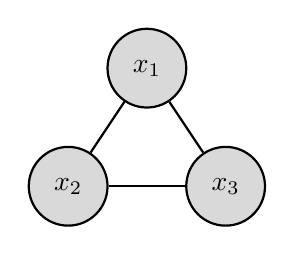
\begin{tikzpicture}[node distance={10mm}, thick,
            main/.style = {draw, circle, minimum size=1cm}]
                \node[main, fill = gray!30] (x1) {$x_1$};
                \node[main, fill = gray!30] (x2) [xshift=-1cm, yshift=-1.5cm] {$x_2$};
                \node[main, fill = gray!30] (x3) [xshift=1cm, yshift=-1.5cm] {$x_3$};

                \draw (x1) -- (x2);
                \draw (x1) -- (x3);
                \draw (x2) -- (x3);
        \end{tikzpicture}
    \end{figure}
    A questo punto colleghiamo ogni vertice $v$ del triangolo con il vertice $\overline{v}$ del grafo
    originale $\mathcal{G}_\phi$.

    Supponendo che $C^{(i)} = (x_1 \lor \overline{x_2} \lor x_3)$, il risultato sarà:
    \begin{figure}[H]
        \centering 
        \begin{tikzpicture}[node distance={10mm}, thick,
            main/.style = {draw, circle, minimum size=1cm}]
                \node[main, fill = gray!30] (v) {$v$};
                \node[main, fill = gray!30] (x1) [below=of v, xshift=-5cm] {$x_1$};
                \node[main, fill = gray!30] (x_1neg) [right=of x1] {$\overline{x_1}$};
                \node[main, fill = gray!30] (x2) [right=of x_1neg] {$x_2$};
                \node[main, fill = gray!30] (x_2neg) [right=of x2] {$\overline{x_2}$};
                \node[main, fill = gray!30] (x3) [right=of x_2neg] {$x_3$};
                \node[main, fill = gray!30] (x_3neg) [right=of x3] {$\overline{x_3}$};

                \draw (v) -- (x1);
                \draw (v) -- (x_1neg);
                \draw (v) -- (x2);
                \draw (v) -- (x_2neg);
                \draw (v) -- (x3);
                \draw (v) -- (x_3neg);

                \draw (x1) -- (x_1neg);
                \draw (x2) -- (x_2neg);
                \draw (x3) -- (x_3neg);

                \node[main, fill = gray!30] (x2_t) [yshift=-4cm] {$x_2$};
                \node[main, fill = gray!30] (x1_t) [below left=of x2_t] {$x_1$};
                \node[main, fill = gray!30] (x3_t) [below right=of x2_t] {$x_3$};

                \draw (x1_t) -- (x2_t);
                \draw (x1_t) -- (x3_t);
                \draw (x2_t) -- (x3_t);

                \draw (x1_t) -- (x_1neg);
                \draw (x2_t) -- (x_2neg);
                \draw (x3_t) -- (x_3neg);
        \end{tikzpicture}
    \end{figure}
    Tale riduzione è polinomiale, poiché considerando una formula con $3m$ letterali, il grafo 
    risultante avrà $3m + 2n + 1$ vertici e $6m + 3n$ archi, dove $n$ è il numero di clausole
    e $m$ è il numero di letterali.

    \begin{description}
        \item[$(\Rightarrow)$] Se la formula $\phi$ in \texttt{NAE-3-SAT} è soddisfacibile, allora esiste un assegnamento
        $a_n \in \{ true, false \}^n$ tale che per ogni $i$, $C^{(i)}(a_n)$ è soddisfatta. Esistono 
        $j,k$ tale che $l_j^{(i)}(a_n) = \texttt{true}$ e $l_k^{(i)}(a_n) = \texttt{false}$.
        Assegneremo quindi la seguente colorazione al grafo $\mathcal{G}_\phi$:
        \[
            C(w) = \begin{cases}
                \texttt{blu} & \text{se } w \text{ è etichettato con } l_i \text{ e } l_i(a_n) = \texttt{true} \\
                \texttt{rosso} & \text{se } w \text{ è etichettato con } l_i \text{ e } l_i(a_n) = \texttt{false} \\
            \end{cases}
        \]
        e fissiamo $C(v) = \texttt{verde}$.
    
        Poiché l'assegnamento era \texttt{NAE-3-SAT}, due di questi letterali di un triangolo avranno
        colori diversi. Mantengo 
        la colorazione dei due vertici con colorazione opposta e modifico la colorazione del terzo vertice
        per garantire che non ci siano due vertici adiacenti con lo stesso colore.
    
        Il risultato sarà il seguente: 
    
        \begin{figure}[H]
            \centering 
            \begin{tikzpicture}[node distance={10mm}, thick,
                main/.style = {draw, circle, minimum size=1cm}]
                    \node[main, fill = green!30] (v) {$v$};
                    \node[main, fill = red!30] (x1) [below=of v, xshift=-5cm] {$x_1$};
                    \node[main, fill = blue!30] (x_1neg) [right=of x1] {$\overline{x_1}$};
                    \node[main, fill = blue!30] (x2) [right=of x_1neg] {$x_2$};
                    \node[main, fill = red!30] (x_2neg) [right=of x2] {$\overline{x_2}$};
                    \node[main, fill = red!30] (x3) [right=of x_2neg] {$x_3$};
                    \node[main, fill = blue!30] (x_3neg) [right=of x3] {$\overline{x_3}$};
    
                    \draw (v) -- (x1);
                    \draw (v) -- (x_1neg);
                    \draw (v) -- (x2);
                    \draw (v) -- (x_2neg);
                    \draw (v) -- (x3);
                    \draw (v) -- (x_3neg);
    
                    \draw (x1) -- (x_1neg);
                    \draw (x2) -- (x_2neg);
                    \draw (x3) -- (x_3neg);
    
                    \node[main, fill = blue!30] (x2_t) [yshift=-4cm] {$x_2$};
                    \node[main, fill = green!30] (x1_t) [below left=of x2_t] {$x_1$};
                    \node[main, fill = red!30] (x3_t) [below right=of x2_t] {$x_3$};
    
                    \draw (x1_t) -- (x2_t);
                    \draw (x1_t) -- (x3_t);
                    \draw (x2_t) -- (x3_t);
    
                    \draw (x1_t) -- (x_1neg);
                    \draw (x2_t) -- (x_2neg);
                    \draw (x3_t) -- (x_3neg);
            \end{tikzpicture}
        \end{figure}
        \item[$(\Leftarrow)$] Supponiamo ora che esista un assegnamento di colori che soddisfa
        \(\mathcal{G}_\phi\) nel problema \texttt{3-COL}. Questo significa che per ogni vertice
        nel grafo, incluso nel triangolo che rappresenta una clausola, i colori devono essere
        assegnati in modo che nessun vertice adiacente abbia lo stesso colore. In particolare,
        ciò implica che in ogni triangolo rappresentante una clausola \(C^{(i)}\), i tre vertici
        (\textit{che rappresentano i tre letterali della clausola}) devono avere almeno due colori
        diversi. Possiamo mappare questo assegnamento di colori indietro a un assegnamento di
        verità in \texttt{NAE-3-SAT} nel seguente modo:
        \begin{itemize}
            \item Assegniamo \texttt{true} ai letterali che sono colorati con il colore, diciamo,
            blu, e \texttt{false} ai letterali che sono colorati con il colore, diciamo, rosso.
        \end{itemize}
        Poiché in \(\mathcal{G}_\phi\) ogni triangolo (\textit{che rappresenta una clausola di \(\phi\)})
        ha vertici di almeno due colori diversi, nessuna clausola di \(\phi\) sarà insoddisfatta.
        Questo perché la condizione di \texttt{NAE-3-SAT} richiede che in ogni clausola, non tutti
        i letterali siano uguali, e l'assegnamento derivato dall'assegnamento di colori garantisce
        esattamente questo. Dunque, \(\phi\) è soddisfacibile in \texttt{NAE-3-SAT}.
    \end{description}
\end{proof}
\subsection{Riduzione di Cook-Levin}
Per dimostrare che \texttt{3-SAT} è \texttt{NP-completo}, abbiamo mostrato che
\texttt{3-SAT} si riduce in tempo polinomiale a \texttt{4-SAT}. Per farlo abbiamo
trasformato ogni clausola $C$ in una clausola $D = (C \lor z)$, dove $z$ è una
variabile ausiliaria. Abbiamo poi trasformato \texttt{4-SAT} in \texttt{3-SAT}.
\[
  (l_1 \lor l_2 \lor l_3 \lor l_4) \rightarrow (l_1 \lor l_2 \lor z) \land
  (\overline{z} \lor l_3 \lor l_4)
\]
Abbiamo poi dimostrato che \texttt{3-SAT} è \texttt{NP-completo}.

La stessa tecnica non ci darebbe informazioni utili per dimostrare che \texttt{2-SAT}
è \texttt{NP-completo}. 

\begin{theorem}
    \texttt{2-SAT} è in \texttt{P}.
\end{theorem}
\begin{proof}
    Per procedere con la dimostrazione consideriamo il problema \texttt{2-SAT} come un problema di ricerca, ovvero cerchiamo un assegnamento di verità che soddisfi la formula $\phi$, mostrando quindi che esiste un algoritmo che in tempo polinomiale risolve il problema.
    
    Data $\phi$, costruiamo un grafo orientato $\mathcal{G}_\phi$ nel seguente modo:
    \begin{itemize}
        \item Per ogni letterale $l_i$ possibile in $\phi$, abbiamo un vertice in $V$.
        \item Per ogni clausola $C$ in $\phi$, aggiungiamo una coppia di archi $(\overline{l_i}, l_j)$ e $(\overline{l_j}, l_i)$.
    \end{itemize}
    Quello che osserviamo è che:
    \begin{itemize}
        \item Se abbiamo il cammino $x_1 \rightarrow x_2 \rightarrow x_3, \dots, x_k \rightarrow y$ in $\mathcal{G}_\phi$,
        un assegnamento che soddisfa la formula $\phi$ e rende $x$ vero, deve mettere a \texttt{true}
        tutti i vertici del cammino.
        \item Se in $\mathcal{G}_\phi$ esiste per una qualche variabile $x$ un cammino $x \rightarrow \overline{x}$
        allora nessun assegnamento che soddisfa la formula $\phi$ può rendere $x$ vero.
        \item Se per qualche variabile $x$ esistono in $\mathcal{G}_\phi$ sia il cammino $x \rightarrow \overline{x}$
        che il cammino $\overline{x} \rightarrow x$, allora non esiste un assegnamento che soddisfa la formula $\phi$.
    \end{itemize}
    Possiamo quindi utilizzare l'algoritmo di \textit{componenti fortemente connesse} per verificare
    se esiste un assegnamento che soddisfa la formula $\phi$.
    
    \begin{algorithm}[H]
        \caption{\texttt{2SAT}}
        \DontPrintSemicolon 
        
        \KwIn{Una formula booleana $\phi$ rappresentata come un insieme di implicazioni in $\mathcal{G}_\phi$}
        \KwOut{\texttt{true} se $\phi$ è soddisfacibile, \texttt{false} altrimenti}
        
        Costruisci il grafo di implicazione $\mathcal{G}_\phi$ per $\phi$ \;
        \ForEach{variabile $x$ in $\mathcal{G}_\phi$}{
            \If{$x \rightarrow \overline{x}$ e $\overline{x} \rightarrow x$}{
                \Return \texttt{false} \Comment{Esiste una contraddizione}
            }
        }
        \Return \texttt{true} \Comment{Nessuna contraddizione trovata, $\phi$ è soddisfacibile}
    \end{algorithm}
    
    Creare il grafo richiede tempo polinomiale, e l'algoritmo di componenti fortemente connesse
    ha complessità $O(V + E)$, dove $n$ è il numero di vertici e $m$ il numero di archi.
    Quindi \texttt{2-SAT} è in \texttt{P}.

    Mostriamo ora che se non troviamo un cammino $x \rightarrow \overline{x}$ o $\overline{x} \rightarrow x$
    allora esiste un assegnamento che soddisfa la formula $\phi$.

    \begin{algorithm}[H]
        \caption{\texttt{2SAT}}
        \DontPrintSemicolon  

        \KwIn{Una formula booleana $\phi$ rappresentata come un insieme di implicazioni in $\mathcal{G}_\phi$}
        \KwOut{Un assegnamento che soddisfa $\phi$}

        \BlankLine
        Costruisci il grafo di implicazione $\mathcal{G}_\phi$ per $\phi$ \;
        \ForEach{variabile $x$ in $\mathcal{G}_\phi$ non ancora assegnata}{
            \If{$x \rightarrow \overline{x}$ in $\mathcal{G}_\phi$}{
                $a_x \gets \texttt{false}$ \;
                \ForEach{percorso $\overline{x} \rightarrow y$ nel $\mathcal{G}_\phi$}{
                    $a_y \gets \texttt{true}$
                }
            }
            \Else{
                $a_x \gets \texttt{true}$ \;
                \ForEach{percorso $x \rightarrow y$ nel $\mathcal{G}_\phi$}{
                    $a_y \gets \texttt{false}$
                }
            }
        }
    \end{algorithm}
    In termini computazionali l'algoritmo richiede tempo $O(2(2V + 2E)\cdot n)$, ovvero due 
    \texttt{BFS} potenzialmente eseguiti su tutti i vertici del grafo, quindi è polinomiale.
\end{proof}

In termini di riduzione, quello che abbiamo dimostrato è che $\texttt{2-SAT} \leq_T \texttt{BFS}$,
dove con il simbolo $\leq_T$ indichiamo una riduzione in tempo polinomiale di Cook-Turing.

\begin{tcolorbox}[title =$\mathbb{A} \leq_T \mathbb{B}$]
    Dati due problemi di decisione $\mathbb{A}$ e $\mathbb{B}$, diciamo che $\mathbb{A} \leq_T \mathbb{B}$
    se esiste un algoritmo in tempo polinomiale per risolvere $\mathbb{A}$ che utilizza chiamate a un
    oracolo per risolvere $\mathbb{B}$.
\end{tcolorbox}
\begin{tcolorbox}[title = Oracolo]
    Un oracolo è un'entità che può rispondere a domande in un solo passo di calcolo, $O(1)$.
\end{tcolorbox}
Notiamo quindi che se un algoritmo risolve $\mathbb{B}$ in tempo polinomiale, allora risolverà
anche $\mathbb{A}$ in tempo polinomiale. 
\begin{theorem}
    Se $\mathbb{A} \leq_T \mathbb{B}$ e $\mathbb{B} \in \texttt{P}$, allora $\mathbb{A} \in \texttt{P}$.
\end{theorem}
Ne consegue che:
\begin{theorem}
    Se $\mathbb{A} \leq_T \mathbb{B}$ e $\mathbb{A} \not \in \texttt{P}$, allora $\mathbb{B} \not \in \texttt{P}$.
\end{theorem}

Inoltre abbiamo che:
\begin{theorem}
    Se $\mathbb{A} \leq \mathbb{B} \implies \mathbb{A} \leq_T \mathbb{B}$.
\end{theorem}
\begin{proof}
    Consideriamo $x$ istanza del problema $\mathbb{A}$, la trasformiamo nell'istanza $y$, ovvero la riduzione applicata 
    a $x$. Applichiamo l'algoritmo per $\mathbb{B}$ all'istanza $y$ e otteniamo la risposta.
    \[
        x \in \mathcal{I}(x) \implies y = R(x) \implies \mathbb{B}(R(x))
    \]
\end{proof}
Si tratta di un caso particolare della riduzione di Cook-Turing, in cui si effettua un'unica chiamata al risolutore,
ma non la si elabora.

